\usetikzlibrary{calc}
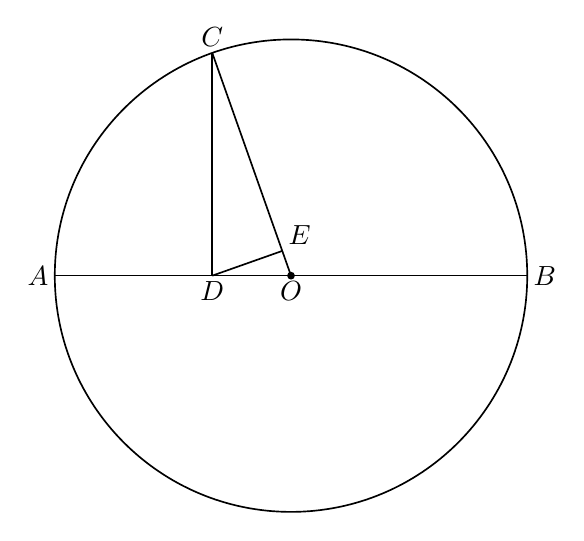
\begin{tikzpicture}[x=1cm,y=1cm,line width=.6pt,font=\normalsize]
\coordinate (O) at (0.0,0.0);
\coordinate (A) at (-3.0,0.0);
\coordinate (B) at (3.0,0.0);
\coordinate (D) at (-1.0,0.0);
\coordinate (C) at (-1.0,2.8284271247461903);
\coordinate (E) at (-0.1111111111111111,0.3142696805273545);
\draw (O) circle[radius=3.0cm];
\draw (A)--(B);
\draw (C)--(D);
\draw (C)--(O);
\draw (D)--(E);
\node[left=2pt,inner sep=0pt] at (A) {$A$};
\node[right=2pt,inner sep=0pt] at (B) {$B$};
\node[above=2pt,inner sep=0pt] at (C) {$C$};
\node[below=2pt,inner sep=0pt] at (D) {$D$};
\node[below=2pt,inner sep=0pt] at (O) {$O$};
\node[above right=2pt,inner sep=0pt] at (E) {$E$};

% Explicit named circle-center points, painted after all region fills.
\fill (O) circle[radius=1.4pt];
\end{tikzpicture}
